\documentclass[aspectratio=169]{beamer}

% Shared preamble for Claude Code slide decks
% Usage: % Shared preamble for Claude Code slide decks
% Usage: % Shared preamble for Claude Code slide decks
% Usage: \input{preamble} after \documentclass[aspectratio=169]{beamer}

\usetheme{default}
\usecolortheme{dove}

\setbeamertemplate{navigation symbols}{}
\setbeamertemplate{footline}{%
  \hfill{\large\insertframenumber\,/\,\inserttotalframenumber}\hspace{0.8em}\vspace{0.5em}%
}

\definecolor{popblue}{RGB}{52, 101, 164}
\definecolor{sampred}{RGB}{204, 0, 0}
\definecolor{paramgreen}{RGB}{0, 140, 70}
\definecolor{lightbg}{RGB}{245, 245, 250}
\definecolor{warnred}{RGB}{180, 40, 40}
\definecolor{orange1}{RGB}{220, 120, 0}
\definecolor{violet1}{RGB}{120, 50, 160}

\setbeamercolor{frametitle}{fg=popblue}
\setbeamercolor{title}{fg=popblue}
\setbeamercolor{block title}{fg=white,bg=popblue}
\setbeamercolor{block body}{bg=lightbg}
\setbeamercolor{block title alerted}{fg=white,bg=warnred}
\setbeamercolor{block body alerted}{bg=lightbg}
\setbeamercolor{block title example}{fg=white,bg=paramgreen}
\setbeamercolor{block body example}{bg=lightbg}

\usepackage{listings}
\usepackage[T1]{fontenc}
\usepackage{hyperref}
\usepackage{tikz}
\usepackage{booktabs}
\usetikzlibrary{shapes, arrows.meta, positioning, calc}

\lstset{
  basicstyle=\ttfamily\scriptsize,
  keywordstyle=\color{popblue}\bfseries,
  stringstyle=\color{paramgreen},
  commentstyle=\color{gray},
  breaklines=true,
  frame=single,
  backgroundcolor=\color{lightbg},
  rulecolor=\color{popblue!30},
  showstringspaces=false,
  columns=fullflexible,
}
 after \documentclass[aspectratio=169]{beamer}

\usetheme{default}
\usecolortheme{dove}

\setbeamertemplate{navigation symbols}{}
\setbeamertemplate{footline}{%
  \hfill{\large\insertframenumber\,/\,\inserttotalframenumber}\hspace{0.8em}\vspace{0.5em}%
}

\definecolor{popblue}{RGB}{52, 101, 164}
\definecolor{sampred}{RGB}{204, 0, 0}
\definecolor{paramgreen}{RGB}{0, 140, 70}
\definecolor{lightbg}{RGB}{245, 245, 250}
\definecolor{warnred}{RGB}{180, 40, 40}
\definecolor{orange1}{RGB}{220, 120, 0}
\definecolor{violet1}{RGB}{120, 50, 160}

\setbeamercolor{frametitle}{fg=popblue}
\setbeamercolor{title}{fg=popblue}
\setbeamercolor{block title}{fg=white,bg=popblue}
\setbeamercolor{block body}{bg=lightbg}
\setbeamercolor{block title alerted}{fg=white,bg=warnred}
\setbeamercolor{block body alerted}{bg=lightbg}
\setbeamercolor{block title example}{fg=white,bg=paramgreen}
\setbeamercolor{block body example}{bg=lightbg}

\usepackage{listings}
\usepackage[T1]{fontenc}
\usepackage{hyperref}
\usepackage{tikz}
\usepackage{booktabs}
\usetikzlibrary{shapes, arrows.meta, positioning, calc}

\lstset{
  basicstyle=\ttfamily\scriptsize,
  keywordstyle=\color{popblue}\bfseries,
  stringstyle=\color{paramgreen},
  commentstyle=\color{gray},
  breaklines=true,
  frame=single,
  backgroundcolor=\color{lightbg},
  rulecolor=\color{popblue!30},
  showstringspaces=false,
  columns=fullflexible,
}
 after \documentclass[aspectratio=169]{beamer}

\usetheme{default}
\usecolortheme{dove}

\setbeamertemplate{navigation symbols}{}
\setbeamertemplate{footline}{%
  \hfill{\large\insertframenumber\,/\,\inserttotalframenumber}\hspace{0.8em}\vspace{0.5em}%
}

\definecolor{popblue}{RGB}{52, 101, 164}
\definecolor{sampred}{RGB}{204, 0, 0}
\definecolor{paramgreen}{RGB}{0, 140, 70}
\definecolor{lightbg}{RGB}{245, 245, 250}
\definecolor{warnred}{RGB}{180, 40, 40}
\definecolor{orange1}{RGB}{220, 120, 0}
\definecolor{violet1}{RGB}{120, 50, 160}

\setbeamercolor{frametitle}{fg=popblue}
\setbeamercolor{title}{fg=popblue}
\setbeamercolor{block title}{fg=white,bg=popblue}
\setbeamercolor{block body}{bg=lightbg}
\setbeamercolor{block title alerted}{fg=white,bg=warnred}
\setbeamercolor{block body alerted}{bg=lightbg}
\setbeamercolor{block title example}{fg=white,bg=paramgreen}
\setbeamercolor{block body example}{bg=lightbg}

\usepackage{listings}
\usepackage[T1]{fontenc}
\usepackage{hyperref}
\usepackage{tikz}
\usepackage{booktabs}
\usetikzlibrary{shapes, arrows.meta, positioning, calc}

\lstset{
  basicstyle=\ttfamily\scriptsize,
  keywordstyle=\color{popblue}\bfseries,
  stringstyle=\color{paramgreen},
  commentstyle=\color{gray},
  breaklines=true,
  frame=single,
  backgroundcolor=\color{lightbg},
  rulecolor=\color{popblue!30},
  showstringspaces=false,
  columns=fullflexible,
}


\title{Introduction to Claude Cowork}
\subtitle{Delegation $\cdot$ Plugins $\cdot$ Scheduling $\cdot$ Research}
\author{mostly Opus 4.6}
\date{}

\begin{document}

\begin{frame}
\titlepage
\end{frame}

% ──────────────────────────────────────────────
\begin{frame}{Previously, on Subagents\ldots}
\begin{columns}[T]
\column{0.5\textwidth}
\begin{block}{Subagents}
Separate Claude instances with their own context window, spawned for specific tasks.
\end{block}

\begin{block}{Built-in Types}
General Purpose (full tools), Explore (fast search), Plan (architecture design).
\end{block}

\begin{block}{Custom Agents}
Define in \texttt{.claude/agents/*.md} with frontmatter: tools, model, isolation, maxTurns.
\end{block}

\column{0.5\textwidth}
\begin{block}{When to Use}
Research, code reviews, parallel work. Avoid for simple tasks or sequential pipelines.
\end{block}

\begin{block}{Advanced Features}
Background execution, worktree isolation, agent teams for multi-session coordination.
\end{block}
\end{columns}
\end{frame}

% ──────────────────────────────────────────────
\begin{frame}{What Is Cowork?}
\textbf{Cowork} = Claude's delegation mode in the desktop app.

Instead of conversation, you \emph{hand off} a complete task and step away.

\bigskip
\begin{center}
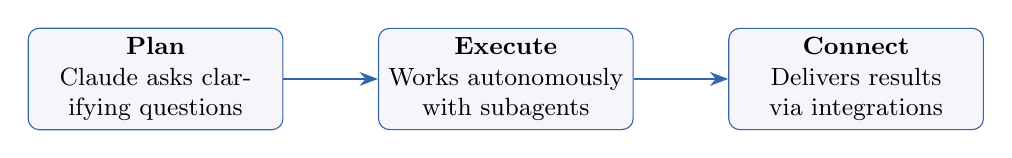
\begin{tikzpicture}[
  node distance=0.6cm and 1.2cm,
  box/.style={rectangle, rounded corners, draw=popblue, fill=lightbg,
              text width=3cm, minimum height=0.9cm, align=center, font=\small},
  arr/.style={-Stealth, thick, popblue}
]
  \node[box] (plan) {\textbf{Plan}\\Claude asks clarifying questions};
  \node[box, right=of plan] (exec) {\textbf{Execute}\\Works autonomously with subagents};
  \node[box, right=of exec] (conn) {\textbf{Connect}\\Delivers results via integrations};
  \draw[arr] (plan) -- (exec);
  \draw[arr] (exec) -- (conn);
\end{tikzpicture}
\end{center}

\bigskip
\textbf{Three modes in Claude desktop:}
\begin{itemize}
  \item \textbf{Chat} --- conversational back-and-forth
  \item \textbf{Cowork} --- delegate and step away
  \item \textbf{Code} --- Claude Code in the IDE
\end{itemize}

\smallskip
\small\textbf{Platforms:} macOS and Windows (since February 2026).
\end{frame}

% ──────────────────────────────────────────────
\begin{frame}{Getting Set Up}
\textbf{Requirements:}
\begin{itemize}
  \item Claude desktop app
  \item Folder access configured (grant access to working directories)
  \item Connectors enabled (Google Drive, Notion, Slack, etc.)
  \item Chrome extension (optional, for web tasks)
\end{itemize}

\bigskip
\begin{alertblock}{Key difference from Chat}
In Cowork, you describe what you want done and \emph{walk away}. Claude will ask clarifying questions only if needed, then execute autonomously.
\end{alertblock}
\end{frame}

% ──────────────────────────────────────────────
\begin{frame}{The Task Loop}
\begin{enumerate}
  \item \textbf{Describe} your task clearly
  \item \textbf{Questions} --- Claude may ask for clarification
  \item \textbf{Step away} --- Claude works with subagents in parallel
  \item \textbf{Open finished work} --- review the deliverables
\end{enumerate}

\bigskip
\textbf{Subagents in Cowork:} {\small(see \emph{Subagents} deck)}
\begin{itemize}
  \item Cowork spawns multiple subagents for parallel execution
  \item Each handles a piece of the overall task
  \item Results are merged into a coherent deliverable
\end{itemize}

\bigskip
\begin{exampleblock}{Example}
``Organize all PDFs in my Downloads folder by topic, rename them with a consistent naming scheme, and create a summary index.''
\end{exampleblock}
\end{frame}

% ──────────────────────────────────────────────
\begin{frame}{Giving Cowork Context}
\begin{columns}[T]
\column{0.5\textwidth}
\textbf{\color{popblue}Projects}
\begin{itemize}
  \item Upload reference files to a project
  \item Claude uses them as knowledge base
  \item Persistent across tasks
\end{itemize}

\bigskip
\textbf{\color{paramgreen}Instructions Panel}
\begin{itemize}
  \item Per-project custom instructions
  \item Tone, format, conventions
\end{itemize}

\column{0.5\textwidth}
\textbf{\color{violet1}Global Instructions}
\begin{itemize}
  \item Apply to all Cowork tasks
  \item Your preferences everywhere
\end{itemize}

\bigskip
\textbf{\color{orange1}In the prompt itself}
\begin{itemize}
  \item Attach files, screenshots
  \item Reference URLs
  \item Be specific about desired output
\end{itemize}
\end{columns}
\end{frame}

% ──────────────────────────────────────────────
\begin{frame}[fragile]{Plugins: Skills + Connectors + Subagents}
\textbf{Plugins} bundle capabilities into installable packages:

\bigskip
\begin{columns}[T]
\column{0.33\textwidth}
\begin{block}{Skills}
Reusable instructions\\(see \emph{Agent Skills} deck)
\end{block}

\column{0.33\textwidth}
\begin{block}{Connectors}
Integrations with\\external services
\end{block}

\column{0.33\textwidth}
\begin{block}{Subagents}
Specialized agent\\definitions
\end{block}
\end{columns}

\bigskip
\textbf{Installation:} Browse the plugin directory (growing catalog), install with one click.

\textbf{Structure:}
\begin{lstlisting}
my-plugin/
  skills/
    data-analysis/SKILL.md
  connectors/
    sheets-connector.json
  agents/
    analyst.md
\end{lstlisting}
\end{frame}

% ──────────────────────────────────────────────
\begin{frame}{Scheduled Tasks \& File Operations}
\textbf{\color{popblue}Scheduled Tasks (\texttt{/schedule}):}
\begin{itemize}
  \item Set up recurring Cowork tasks
  \item Define cadence (daily, weekly, custom)
  \item Manage and monitor from the app
\end{itemize}

\bigskip
\textbf{\color{paramgreen}File \& Document Tasks:}

Follow the prompt pattern: \textbf{Input $\to$ Transformation $\to$ Output}

\begin{exampleblock}{Examples}
\begin{itemize}
  \item ``Take these 20 customer emails, extract feature requests, create a prioritized spreadsheet''
  \item ``Read all markdown files in docs/, fix formatting, add missing headers''
  \item ``Convert this PDF report into a slide deck with key findings''
\end{itemize}
\end{exampleblock}
\end{frame}

% ──────────────────────────────────────────────
\begin{frame}{Research \& Analysis at Scale}
Cowork excels at \textbf{volume, parallelism, and in-place computation}.

\bigskip
\textbf{Tips for effective research prompts:}
\begin{itemize}
  \item Ask \textbf{sharp, specific questions} (not broad/vague)
  \item Specify the \textbf{output format} you want
  \item Provide \textbf{source materials} or point to directories
  \item Let Cowork parallelize across subagents
\end{itemize}

\bigskip
\begin{block}{Permissions \& Model Choice}
\begin{itemize}
  \item Cowork runs in \textbf{isolated execution} --- controlled access
  \item Review outputs before acting on them
  \item Model choice: \textbf{Opus} (complex), \textbf{Sonnet} (balanced), \textbf{Haiku} (fast/cheap)
\end{itemize}
\end{block}
\end{frame}

% ──────────────────────────────────────────────
\begin{frame}{Computer Use}
\textbf{Claude can control your computer} --- open apps, navigate browsers, fill forms, click UI elements.

\bigskip
\textbf{How it works:}
\begin{enumerate}
  \item Grant Claude screen and input access
  \item Describe the task (e.g.\ ``book a meeting with Alex on Tuesday'')
  \item Claude navigates the screen autonomously
  \item Review and confirm actions
\end{enumerate}

\bigskip
\begin{columns}[T]
\column{0.5\textwidth}
\begin{exampleblock}{Use cases}
\begin{itemize}
  \item Fill out forms across multiple tools
  \item Navigate legacy systems without APIs
  \item Automate repetitive desktop workflows
\end{itemize}
\end{exampleblock}

\column{0.5\textwidth}
\begin{alertblock}{Limitations}
\begin{itemize}
  \item macOS primary; Windows support expanding
  \item Review actions before confirming
  \item Not suitable for high-stakes inputs
\end{itemize}
\end{alertblock}
\end{columns}
\end{frame}

% ──────────────────────────────────────────────
\begin{frame}{Summary}
\begin{block}{Key Takeaways}
\begin{itemize}
  \item Cowork = \textbf{delegation mode}: describe task, step away, get results
  \item Task loop: Describe $\to$ Clarify $\to$ Execute $\to$ Deliver
  \item Context via: projects, instructions panel, global settings, inline
  \item Plugins bundle skills + connectors + subagents
  \item \texttt{/schedule} for recurring tasks
  \item File tasks: Input $\to$ Transformation $\to$ Output pattern
  \item Computer Use: desktop automation (macOS; review before confirming)
  \item Research: sharp questions, specified format, parallelized execution
\end{itemize}
\end{block}

\vfill
\centering
\Large\color{popblue} Questions?
\end{frame}

\end{document}
